\documentclass[11pt]{article}
\usepackage[utf8]{inputenc}
\usepackage{fourier}
\usepackage[T1]{fontenc}
\usepackage{natbib}
\usepackage[top=2.5cm, bottom=2.5cm, left=2.5cm, right=2.5cm]{geometry}
\usepackage{graphicx}
\usepackage{authblk}
\usepackage{hyperref}
\usepackage{fancyref}
\usepackage{listings}
\usepackage{abstract}
\renewcommand{\abstractname}{}    % clear the title
\renewcommand{\absnamepos}{empty} 
\setlength\parindent{0pt}

\sloppy

\title{\textbf{Machine Learning and Data Mining with Apache Spark}}
\author{Benjamin Fovet, Maxime Gasque, François Horel, Héloïse Hourquebie, Abderrahman Lahjouji, Anass Seddiki}
\affil{\texttt{\{bfovet, mgasque, fhorel, hhourquebie, alahjouji, aseddiki\} @enseirb-matmeca.fr}}
\date{}

\begin{document}

\maketitle

\begin{abstract}
\textbf{Abstract.} This paper deals with the concepts of \textbf{\textit{machine learning}} and \textbf{\textit{data mining}} social networks, which are increasingly useful for businesses to know the consumers' sentiment towards their brand. This project, intended for use by engineers at \textsf{Orange France}, focuses on the development of a micro-services architecture built around the open source cluster computing framework, \textsf{\textbf{Apache Spark}}. Thanks to is distributed model, \textsf{Spark} can process massive amounts of data stored in databases as well as real time data streamed from social networks. Data is then stored in a cluster database and exposed by an API (Application Programming Interface) for users to see them in real time.
\end{abstract}

\section{Context}
% What is Big Data ? (short intro)
Big data [1] is a term used to designate data that is not only too voluminous to fit in a standard database, but is also too diverse and appears at such speed that it cannot be processed using mainstream systems. 
\vskip 9pt

% Orange wants to use Apache Spark
Currently, \textsf{Orange} is a company already working on big data applications and is interested in using emerging big data technologies. More precisely, among those technologies available today, \textsf{Apache Spark} is the most promising one thanks to its processing performances that makes it well suited to machine learning algorithms.

% What is Apache Spark ? What are the possibilities ? How does it work ?
\subsection{Apache Spark}
\label{apache spark}
\textsf{Apache Spark} is a distributed and highly scalable system, providing the ability to develop applications using languages like \textsf{Java}, \textsf{Scala} (the language used to write \textsf{Spark} itself), \textsf{Python} and \textsf{R}. It was originally developed at the University of California, Berkeley and donated to the Apache Software Foundation in 2013.

Contrary to existing distributed computing software for processing very large data sets, such as \textsf{Apache Hadoop}, \textsf{Spark} is based on an in-memory programming model, instead of using the \textsf{MapReduce} [2] disk-based model, allowing it to be faster and more flexible. For instance, \textsf{Spark} can sort 100 TB of data three times faster and with ten times fewer machines than \textsf{MapReduce} [3].
\vspace{9pt}

\textsf{Spark} consists of four main interoperable components. The figure \ref{spark-stack} shows the modules built on top of the \textsf{Spark Core}.

\newpage
\begin{figure}[h!]
    \centering
    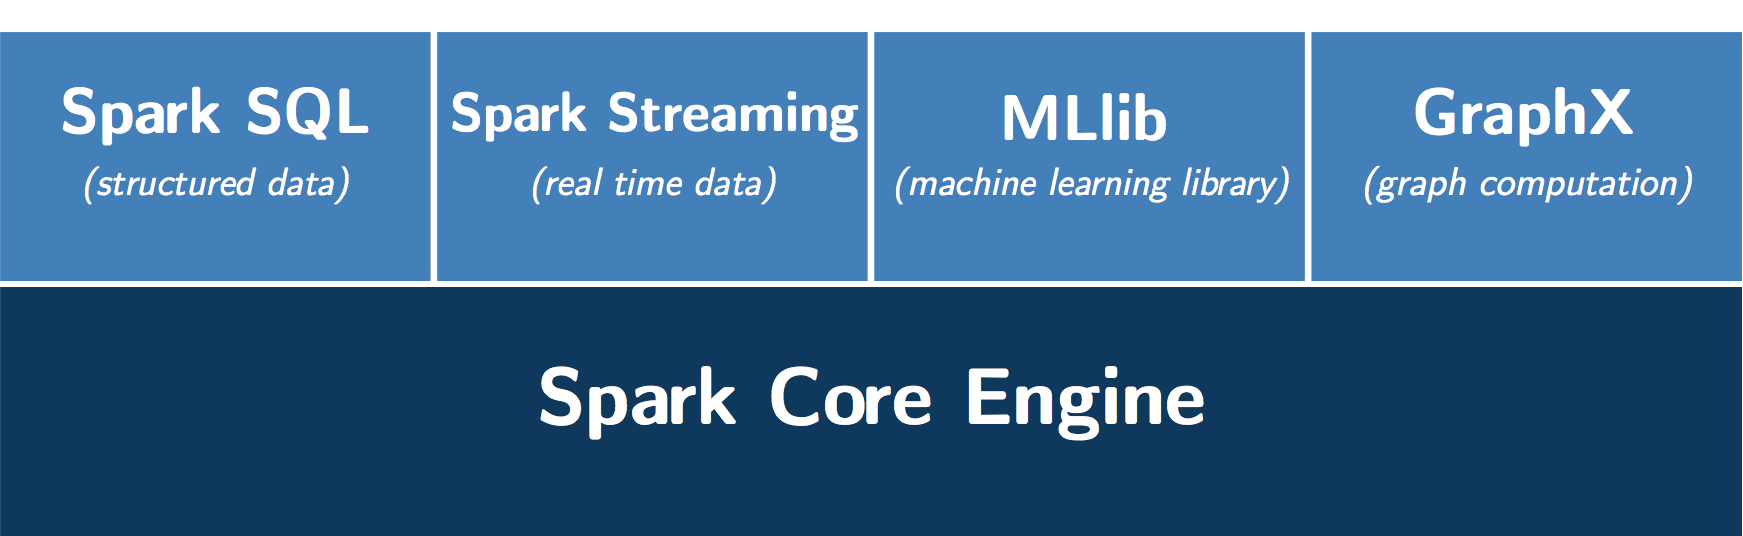
\includegraphics[scale=0.2]{img/spark-stack.eps}
    \caption{The Spark stack}
    \label{spark-stack}
\end{figure}

\textsf{Spark Core} is the foundation of the \textsf{Spark} project and contains features such as task scheduling, memory management, fault recovery and more. On top of that lies four modules.
\textsf{\textbf{Spark SQL}} is \textsf{Spark}'s package for working with structured data which allows \textsf{SQL} queries on many sources of data.
\textsf{\textbf{Spark Streaming}} leverages \textsf{Spark Core} capabilities to enable processing of live streams of data. It is used extensively in this project for fetching data from social networks.
\textsf{\textbf{MLlib}} is a library containing machine learning algorithms that can be applied to compute statistical models from data.
Finally, \textsf{\textbf{GraphX}} is another library for manipulating graphs and performing graph computations. 

% Our goal is to demonstrate Spark capabilities, effectiveness and usability through use cases
\subsection{Using Spark in real world scenarios}
The goal of this project is to demonstrate \textsf{Spark} capabilities, effectiveness and usability. At first, requirements were not clearly defined as this project is mainly aimed at exploring what can be done with \textsf{Spark}, but they had to match certain expectations from \textsf{Orange}. These requirements, introduced in the next section, take the shape of use cases as well as \textsf{Spark} integration with other tools.

\section{Developed use cases}
% Video use case
\subsection{Estimating the crowd in Orange stores}

In the way \textsf{Google} shows rush hours of stores and businesses [4], the first use case consists of analyzing videos to deduce when customers are more likely to visit \textsf{Orange} stores. \textsf{OpenCV} was used...

% Social networks use case
\subsection{Data mining social networks}

\subsubsection{Identifying useful sources}

Social networks are a highly valuable source of information about consumers relationship towards a brand. For instance, \textsf{Orange} uses \textsf{Facebook} through two pages: \href{https://www.facebook.com/Orange.France/?ref=ts}{\textsf{Orange}} and \href{https://www.facebook.com/sosh/?fref=ts}{\textsf{Sosh}}, manages several \textsf{Twitter} accounts: \href{https://twitter.com/orange}{\textsf{@orange}} and \href{https://twitter.com/Orange_France}{\textsf{@Orange\_France}} for general communication about \textsf{Orange}, \href{https://twitter.com/Sosh_fr}{\textsf{@Sosh\_fr}} and \href{https://twitter.com/Orange_conseil}{\textsf{@Orange\_conseil}} as after-sales service accounts. Moreover, consumers can access forums at \href{https://communaute.orange.fr}{\url{communaute.orange.fr}}. These sources are used for fetching live data and feeding \textsf{Spark} with them.

\subsubsection{Spark applications}

As said in section~\ref{apache spark}, \textsf{Spark} applications can be written in several languages: \textsf{Java}, \textsf{Python} or \textsf{Scala}. \textsf{Scala} was initially chosen since \textsf{Spark} itself is developed in \textsf{Scala} and it is also less verbose than \textsf{Java} code. Furthermore, \textsf{Java} and \textsf{Scala} applications have the advantage of being compiled and packaged into an \textsf{\textbf{Uber-JAR}}. \textsf{\textbf{JAR}} (\textsf{Java} ARchive) is a package file format used to aggregate class files required for an application to run, and an \textsf{Uber-JAR} is a \textsf{JAR} that not only contains the application code but also embeds its dependencies as well. This way, the application only needs to be submitted with the \textsf{Uber-JAR} file to \textsf{Spark} to be executed.

Applications are also separated by sources, allowing a more flexible development and release to production as well as a reduction of risks. Indeed, \textsf{Facebook} and \textsf{Twitter} have their own independent API services and having issues with one will not impact the other. This structure also leads to a better bug tracking management with having the bug-free application uninterrupted.

\subsubsection{Sentiment analysis}

Sentiment analysis refers to the use of natural language processing and text analysis to identify and extract subjective information in source materials. It aims at classifying the polarity of a given text — whether the expressed opinion is positive, negative, or neutral. 
Based on the source, sentiment analysis is applied to tweets on \textsf{Twitter}, posts on \textsf{Facebook}, and thread titles and messages on forums.

\paragraph{Dictionary-based approach}

The first approach consists of deciding whether a text is positive, negative or neutral by looking at words in isolation, giving positive points for positive words and negative points for negative words found in two separate dictionaries and then summing up these points.

The following workflow example is based on a real tweet from an \textsf{Orange} consumer.

\begin{figure}[h!]
    \centering
    
\includegraphics[scale=0.6]{img/tweet1.png}
    \caption{Tweet from a user to \textsf{@Orange\_conseil}}
    \label{tweet1}
\end{figure}

The first step is to tokenize the text, translating a sentence into a list of independant words. This is done using the  \href{https://github.com/stanfordnlp/CoreNLP/blob/master/src/edu/stanford/nlp/international/french/process/FrenchTokenizer.java}{\texttt{FrenchTokenizer}} class, part of the \href{https://stanfordnlp.github.io/CoreNLP}{\textsf{\textbf{Stanford CoreNLP}}} suite of Natural Language Processing tools [5]. Along with tokenizing a text, common words with no interesting meaning such as "le", "dans", "à" also known as "stop words" are filtered out to produce the following list of meaningful words.

\vspace{9pt}
\begin{figure}[h!]
    \centering
    \textsf{connexion, internet, vraiment, instable, moment, souvent, aucun, accès, internet, normal}
    \caption{Words after tokenization}
    \label{tokens}
\end{figure}

Next, each word in the above list is looked up in the positive and negative words dictionaries. If found, the weight associated with a negative or positive sentiment, depending on which dictionary the word has been found in, is increased by an increment of one.

In the above tweet, the words \textit{instable, aucun} can be found in the negative words. The word \textit{normal} is not considered positive nor negative because of the context. In order to label it accordingly, a look behind processing has to be implemented to detect the presence of the word \textit{pas}. The structure \textit{pas normal} would then be labeled as negative meanwhile \textit{normal} would be positive.

Finally, the sentiment for the whole tweet is given by computing the difference between the positive weight and the negative weight. A sentiment score equal to 0 is associated with "NEUTRAL", while positive scores are marked as "POSITIVE" and negative scores as "NEGATIVE". Consequently, the example tweet has a negative weight of 2 and a positive weight of 0, labeling it as negative.

\vspace{9pt}
This method is far from perfect since it gives a sentiment based on separate words instead of the context of a sentence. The sentiment analysis annotator from \textsf{Stanford CoreNLP} was tested before implementing this technique and although it yields more accurate results based on a large grammar treebank, it is only available for English text analysis.

\paragraph{Machine learning-based approach}

Thanks to \textsf{Spark}'s Machine Learning library \textsf{MLlib}, classification algorithms can be applied to analyze tweets. In this approach, the Naive Bayes [6] algorithm, a probabilistic classifier based on Bayes' theorem, and the Random Forest [7] algorithm, an ensemble of decision trees for binary and multiclass classification, are implemented through two steps: train and predict.

\vspace{9pt}
Training the data requires having a set of tweets already classified by hand, with 1 meaning positive and 0 meaning negative. This data set is then loaded and 80\% of the data is split into training data, used to train the classifier model, while 20\% is split into testing data, used to assess the performance and the accuracy of the trained model.
With these algorithms, 74\% of the 1343 tweets is correctly classified. According to the computed results below, the Random Forest algorithm is slightly more accurate than the Naive Bayes algorithm yet it is less time efficient. % Add detail about trees options ?

\begin{center}
\begin{tabular}{|l|c|c|}
  \hline
  Algorithm & Naive Bayes & Random Forest \\
  \hline
  Accuracy & 74.04\% & 77.39\% \\ \hline
  Training duration (ms) & 623 & 14266 \\ \hline
  Testing duration (ms) & 13 & 193 \\
  \hline
\end{tabular}
\end{center}

Predicting data classification is then possible by applying the previous trained model.

\subsubsection{Specific computed indicators}

\paragraph{Twitter}

For \textsf{Twitter}, the response time of a tweet addressed to after sales accounts such as \textsf{@Sosh\_fr} and \textsf{@Orange\_conseil}, the number of retweets for a tweet, the number of tweets per second as well as a ranking of trending hashtags are indicators computed from tweets data.

\paragraph{Facebook}

\paragraph{Orange forums}

Scraping \textsf{Orange} forums web pages was done in \textsf{Scala}, for better integration with \textsf{Spark}, using \href{https://github.com/ruippeixotog/scala-scraper}{\texttt{scala-scraper}} [8] which provides a powerful library for scraping \textsf{HTML}. At first, each subforum's first page is scraped to fetch the threads' title, link, date and messages. Then the last thread's date is compared to the current system's time. If the two match, data is stored in \textsf{Cassandra}. This is done every minute for real time streaming. Following the same pattern, the number of unanswered topics can be computed. 

% Every component of our architecture
\section{Building a microservices architecture}

% Presentation and schema first

Microservices pattern is an architectural style in which large complex software applications are broken down into a collection of small, independent, loosely coupled processes. This helps upgrading, modifying or changing one service instead of taking down the entire system. As shown in the figure below, this project is composed of several services communicating with each other, which are presented in the next sections.

\begin{figure}[h!]
    \centering
    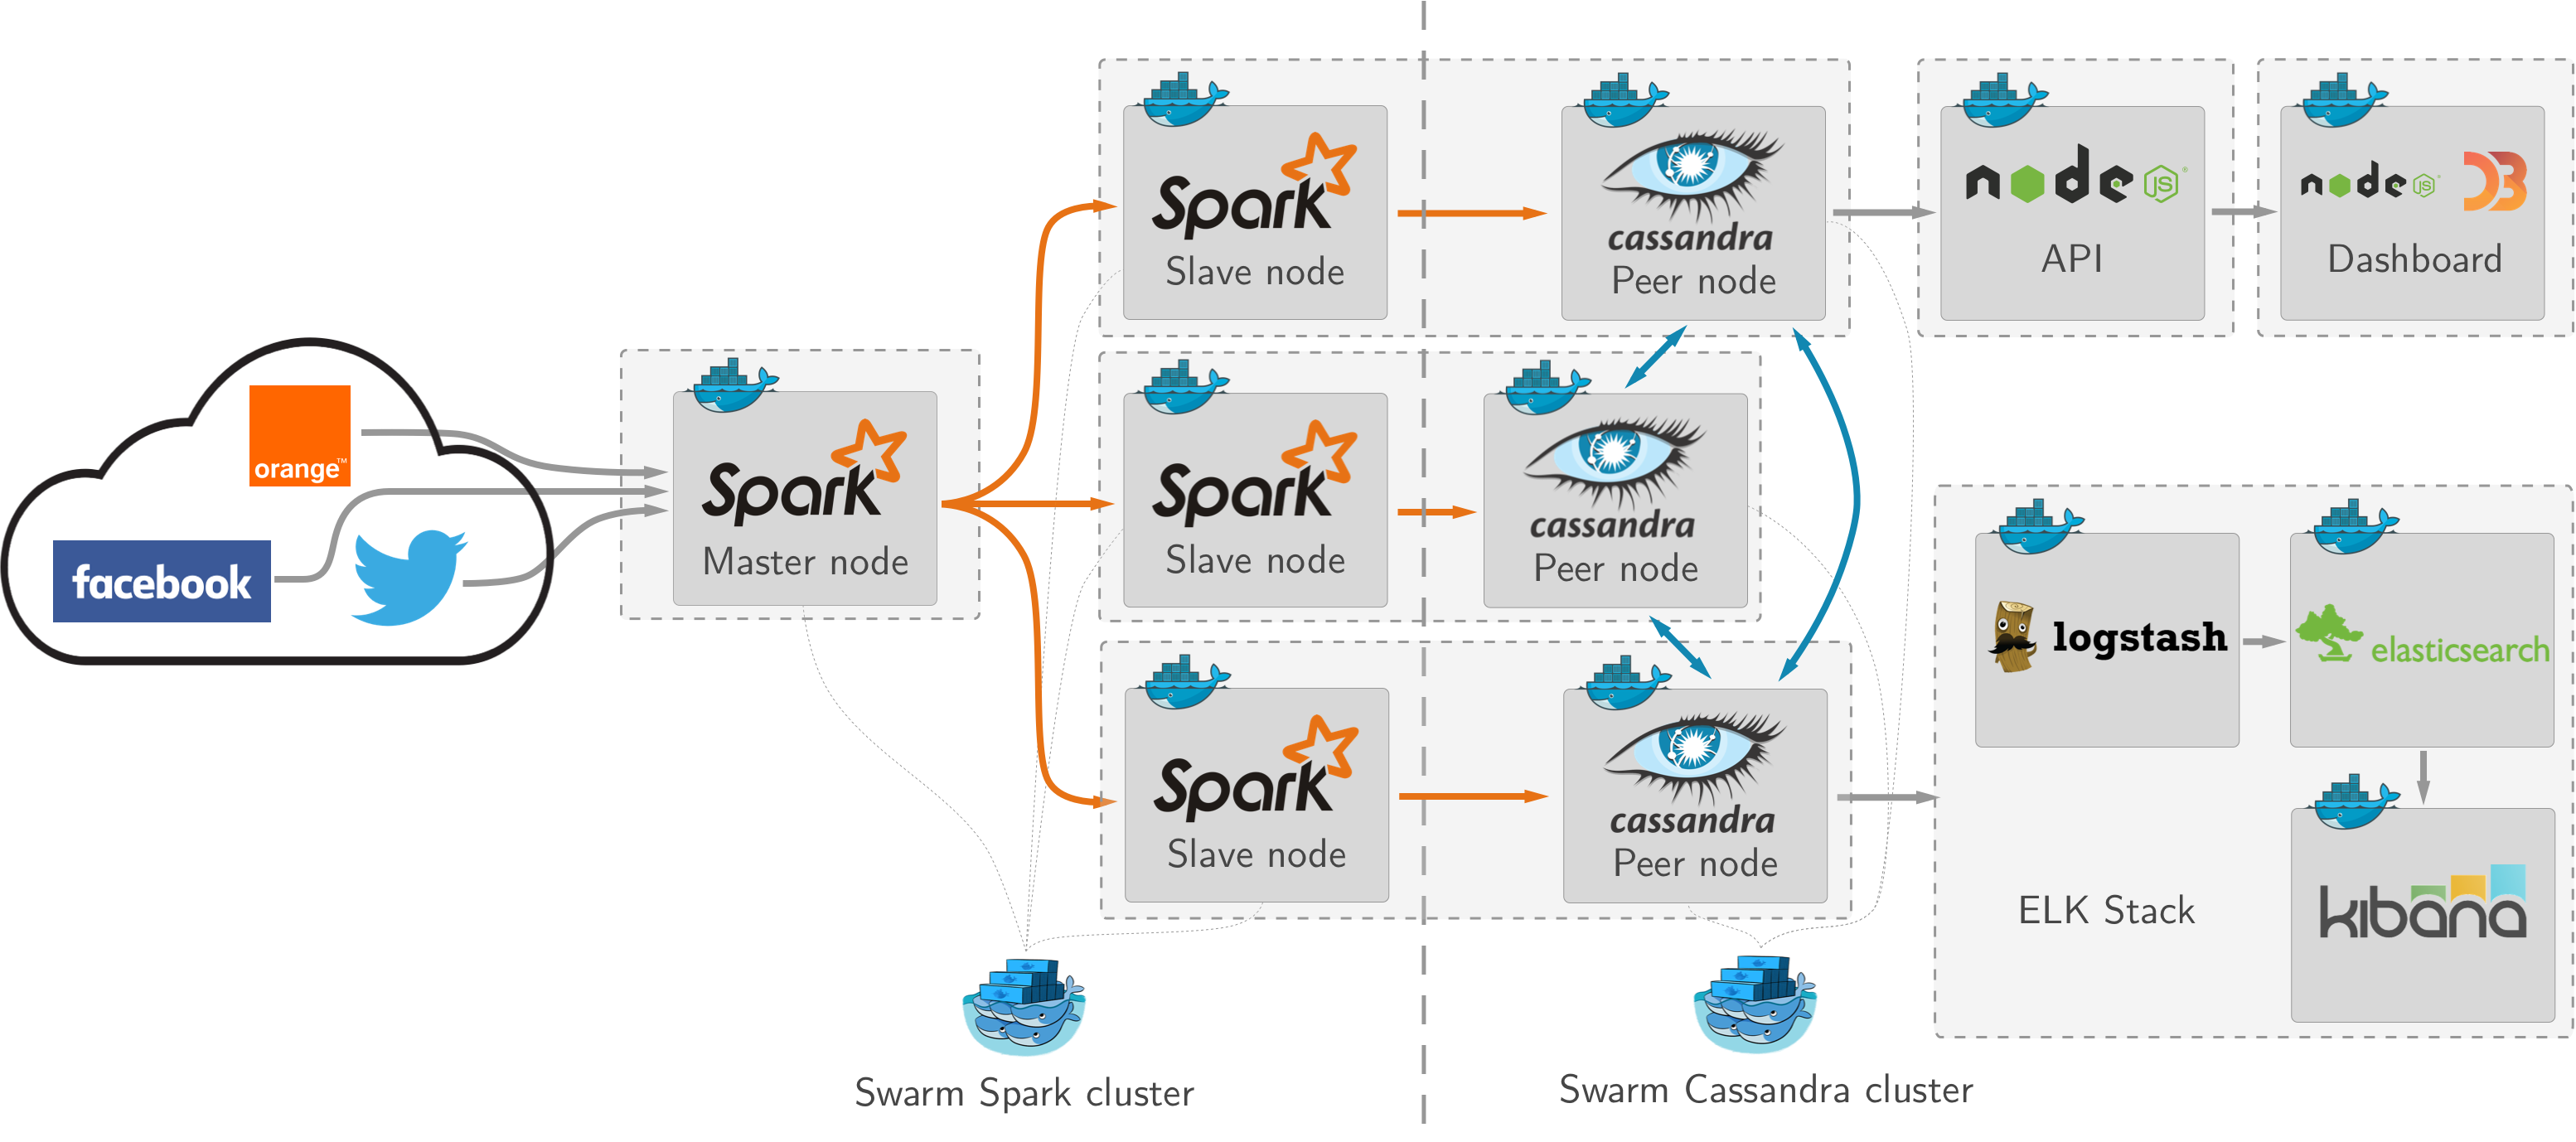
\includegraphics[scale=0.15]{img/archi.png}
    \caption{Deployed infrastructure}
    \label{infra}
\end{figure}

\subsection{Docker}

To facilitate the deployment of each application, \textsf{Docker} is the ideal technology. It automates the deployment of applications inside containers, isolated from the host and other containers by leveraging features of the \textsf{Linux} kernel. \textsf{Docker} containers wrap up a piece of software in a complete filesystem with its dependencies – ensuring that it will run consistently across all environments. In terms of virtualization, \textsf{Docker} uses the features of the host OS (Operating System) instead of requiring an hypervisor and a guest OS like a virtual machine.

%\begin{figure}[h!]
%    \centering
%    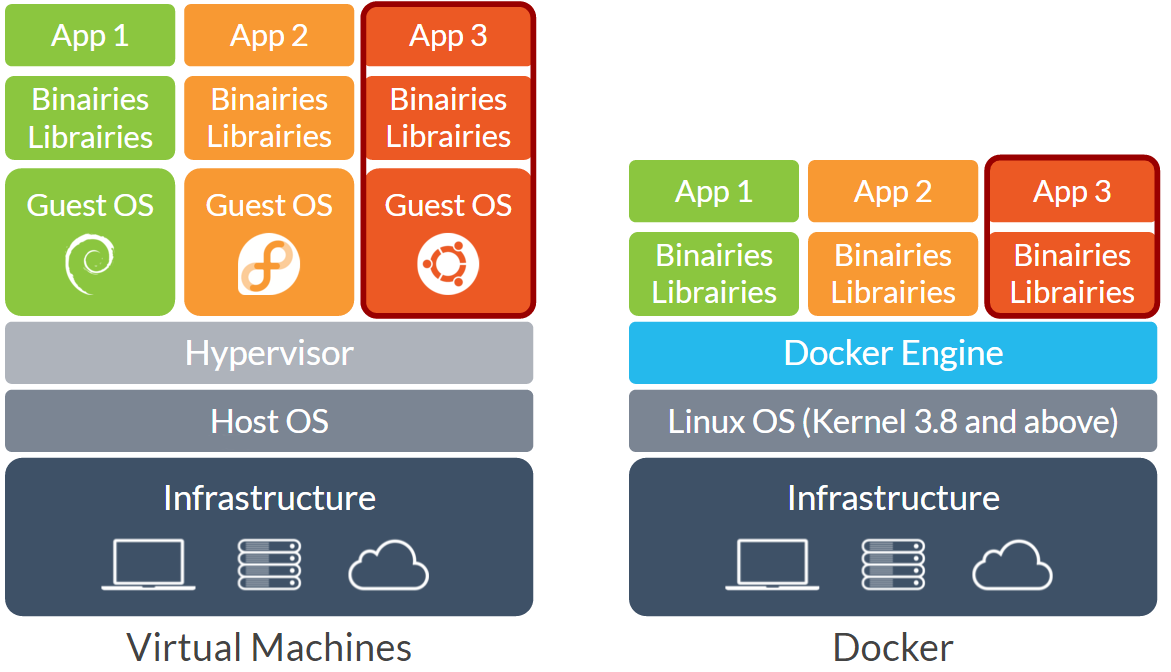
\includegraphics[scale=0.3]{img/docker-vs-vm.png}
%    \caption{Comparison between VMs and Docker}
%    \label{docker-vs-vm}
%\end{figure}

The \textsf{Spark} cluster is deployed with \textsf{Docker Compose} [9] and both clusters are orchestrated with \textsf{Docker Swarm} [10].

\subsection{Spark cluster}

\textsf{Spark} follows the master-slave model and it is composed of a master which schedules and shares jobs between one or more workers.

\subsection{Cassandra cluster}

\textsf{Apache Cassandra} is a \textsf{NoSQL} open-source distributed database system. It is designed to handle large amount of data replicated across servers in a cluster. Each node is installed on the same machine as the \textsf{Spark} workers in order to optimize access to the database and minimize network latency.

\paragraph{Parameters}

Ensuring reliability and fault tolerance on multiple nodes is possible by setting the replication factor according to the number of nodes in the cluster. For instance, three nodes (A, B, C) are deployed for this project. 

With a replication factor of 3, the QUORUM level (rounded down to a whole number) is (replication factor/2) + 1 = 2 which means the cluster can tolerate 1 node down. Besides, each node holds 100\% of the data. This allows a client to write data to A and read the exact replica from B.

Furthermore, consistency is configured to use the QUORUM level with the following \textsf{CQL} (\textsf{Cassandra} Query Language) [11] command:

\begin{lstlisting}[xleftmargin=5cm]
    CONSISTENCY QUORUM;
\end{lstlisting}
With a replication factor of 3, this ensures that 2 nodes are always written and 2 nodes are always read.

\paragraph{Data schema}

Data is stored in different keyspaces related to the aggregated sources: \textit{twitter\_streaming}, \textit{facebook} and \textit{forums} respectively for \textsf{Twitter}, \textsf{Facebook} and \textsf{Orange} forums.

For example, tweets are stored in a table called tweets with extracted fields from \textsf{Twitter} as well as computed ones: response\_time and sentiment.
          
Two other tables are used for storing the velocity in tweets/min (freq) and the most popular hashtags (trends).

\subsection{API}

A RESTful API, developed with \textsf{NodeJS}, is connected to \textsf{Cassandra} to make data available for visualization. 
Its documentation is written with \textsf{Swagger} [12] for a better visual representation.

\begin{figure}[h!]
    \centering
    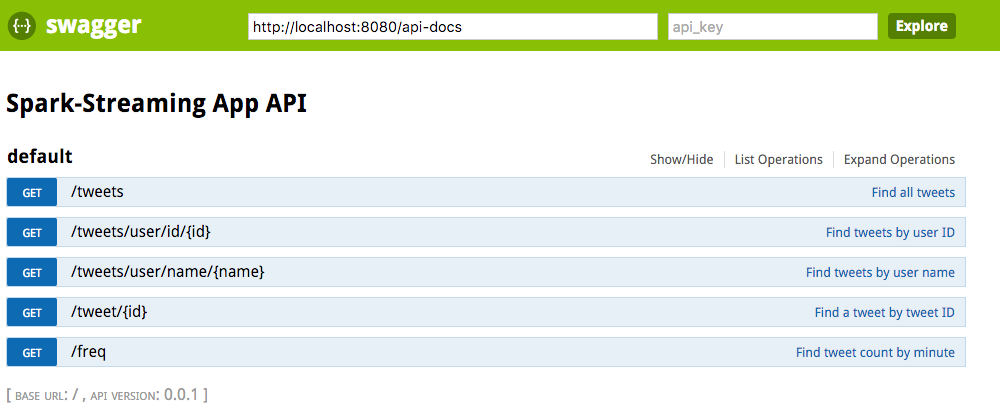
\includegraphics[scale=0.4]{img/api-docs.png}
    \caption{API documentation available at \url{{API_IP_ADDRESS}:8080/docs}}
    \label{socket}
\end{figure}

The \textsf{NodeJS} driver for \textsf{Cassandra} [13] is implemented for streaming data stored in the database to the API.

Along with this API, another \textsf{NodeJS} web server has been developed to serve a web dashboard, using \textsf{D3.js} [14] for charts. When a client loads the page, data is pushed from the API to the dashboard using \textsf{Socket.io} [15].

\begin{figure}[h!]
    \centering
    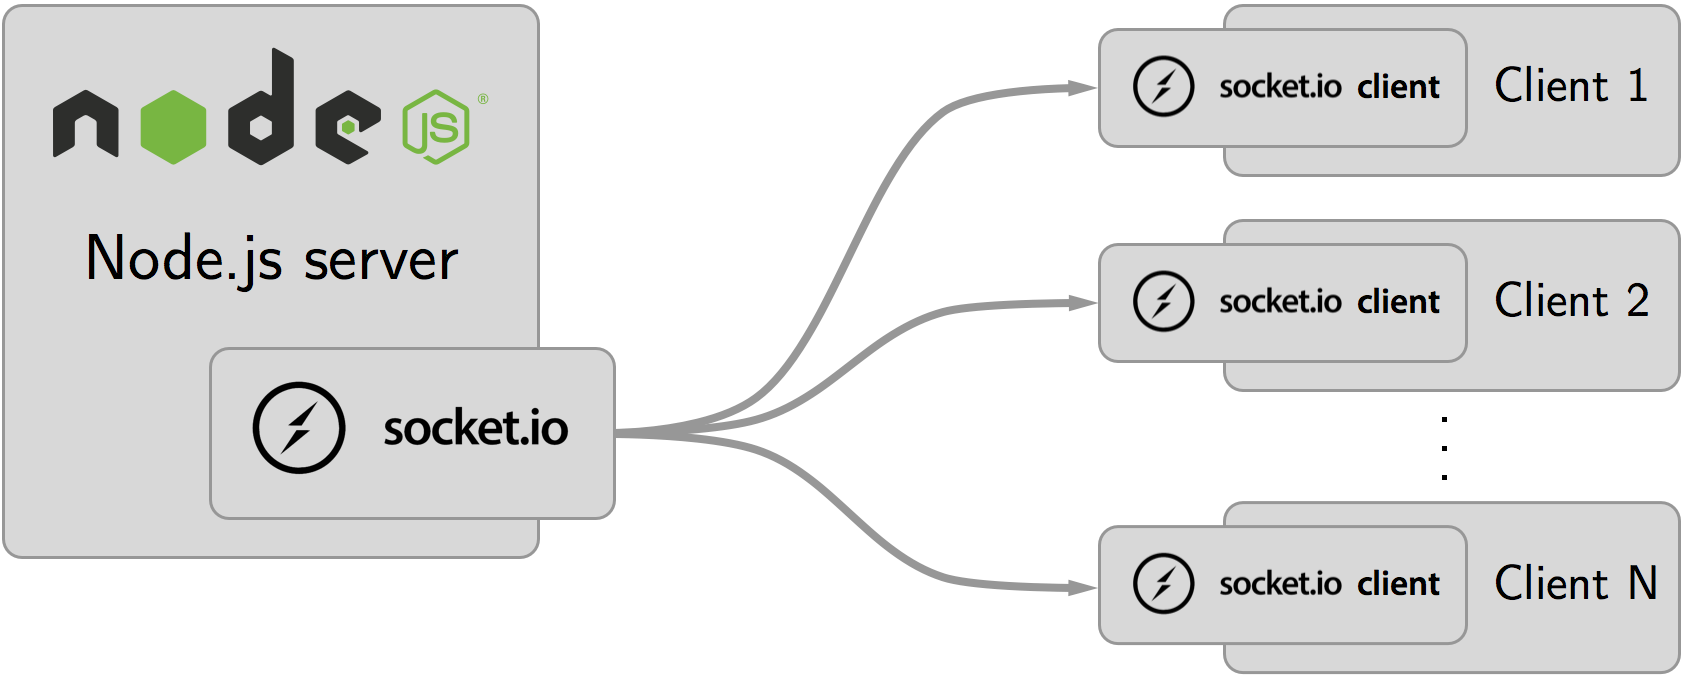
\includegraphics[scale=0.12]{img/api-dashboard-socket.png}
    \caption{Realtime communication between clients and the server with \textsf{Socket.io}}
    \label{socket}
\end{figure}

\subsection{ELK stack}

In parallel, the \textsf{ElasticSearch} - \textsf{Logstash} - \textsf{Kibana} stack is tested as a turnkey solution to replace \textsf{Cassandra}, the API and the web dashboard. % à détailler

\section{Organization and Management}

\subsection{Methodology}

Agile software methodology was an efficient way of organizing this project where objectives were not accurate and stable at the beginning. The development was split in sprints (or iteration) of 3 weeks (See appendices).
Moreover, short-term sprints allowed a part of the team to stop the video processing development before running low on budget (in hours).

The clients were actively involved in the process and meetings were planned every week when possible to demonstrate and review new features. The progress of the project could be followed thanks to weekly progress reports available at \url{bfovet.vvv.enseirb-matmeca.fr/reporting_projet}.

A team charter was first written to define the organization and the values shared by the team during this project.

\subsection{Tools}

The project was managed on \textsf{Trello}. For each sprint, three boards (To do, In progress, Done) were used to sort tasks.
Progress and meeting reports, resources, tutorials as weel as management documents were shared on \textsf{Google Drive}.
\textsf{GitHub} was used for source code hosting and issue tracking. Each service/use case has its own repository, available at \url{https://github.com/t3g7}.
Applications were unit tested with \textsf{Travis CI}, a continuous integration service used to build and test projects hosted at \textsf{GitHub}. Each time a team member pushed code to \textsf{GitHub}, a test build was triggered on \textsf{Travis CI}.
After a successful test on \textsf{Travis CI}, the resulting built \textsf{Docker} image was uploaded to the \textsf{Docker Hub}, a cloud hosted service for \textsf{Docker} image repositories.

\subsection{Issues}

Early in the project, data privacy issues were faced. A use case about analyzing customers logs was considered yet data had to be anonymized in the first place. Also, because access to \textsf{Orange} data was restricted, it was decided to focus on alternative sources of data: social networks and open source data sets.

Moreover, many technical issues had to be solved or bypassed. At first, \textsf{Scala} was a new language with a particular syntax to be assimilated and machine learning and big data were concepts not addressed classes. Installing and configuring \textsf{Apache Spark} took several hours to be complete. Because a microservices architecture was preferable to be dealt with, many different parts hat to be developed and then integrated together.

The sprint involving video processing had to be abandoned due to an overtime risk. Its integration with \textsf{Spark} was indeed too complex since it involved machine learning on images as well as streaming large amounts of data in real time.

\section{Conclusion}

The project consists of applications and services developed around \textsf{Apache Spark}, itself a useful piece of software for processing large amounts of data from various aggregated sources in real time, whether they are databases or online APIs. Development of such applications is relatively simple thanks to a rich ecosystem, including many libraries, bindings for different popular languages and an active community.
\vspace{4pt}

Though not completed, it would have been possible with enough allocated time to compute stores rush hours with video processing by combining \textsf{OpenCV} and \textsf{Spark}. Objectives of this use case were defined as identifying overcrowded stores and predicting popular times to shorten customers waiting time.
\vspace{4pt}

Finally, applications for data mining social networks - \textsf{Twitter}, \textsf{Facebook} and \textsf{Orange} forums - are a tool to help community managers to focus on unanswered questions of customers on after-sales accounts and offer a global point of view on trends and sentiment towards the brand from uncorrelated data.
\vspace{4pt}

While \textsf{Spark} continues to be heavily developed and maintained, next generation software for big data processing are being released. \textsf{Apache Flink} [16] is still in a beta state (0.10.1 - 27 November 2015) and it is focused on streaming making it equivalent to the \textsf{Spark Streaming} module.

\section{References}
\bibliographystyle{plain}
\bibliography{references}

[1] \textit{Big data now, 2014 edition}. O'Reilly Media, 2015
\vspace{1pt}

[2] \url{https://wiki.apache.org/hadoop/MapReduce}
\vspace{1pt}

[3] "Spark wins Daytona Gray Sort 100TB Benchmark." \url{https://spark.apache.org/news/spark-wins-daytona-gray-sort-100tb-benchmark}. 5 November 2014
\vspace{1pt}

[4] Business popular times on Google. \url{https://support.google.com/business/answer/6263531?hl=en}
\vspace{1pt}

[5] Manning, Christopher D., Mihai Surdeanu, John Bauer, Jenny Finkel, Steven J. Bethard, and David McClosky. 2014. The Stanford CoreNLP Natural Language Processing Toolkit In \textit{Proceedings of the 52nd Annual Meeting of the Association for Computational Linguistics: System Demonstrations}, pp. 55-60. \url{http://nlp.stanford.edu/pubs/StanfordCoreNlp2014.pdf}
\vspace{1pt}

[6] Naive Bayes, \url{https://spark.apache.org/docs/latest/mllib-naive-bayes}
\vspace{1pt}

[7] Random Forest, \url{https://spark.apache.org/docs/latest/mllib-ensembles#random-forests}
\vspace{1pt}

[8] Rui Gonçalves, scala-scraper on GitHub, \url{https://github.com/ruippeixotog/scala-scraper}
\vspace{1pt}

[9] Docker Compose, \url{https://docs.docker.com/compose}
\vspace{1pt}

[10] Docker Swarm, \url{https://docs.docker.com/swarm}
\vspace{1pt}

[11] CQL, \url{http://docs.datastax.com/en/cql/3.1/cql/cql_intro_c}
\vspace{1pt}

[12] Swagger, \url{http://swagger.io}
\vspace{1pt}

[13] DataStax, nodejs-driver on GitHub, \url{https://github.com/datastax/nodejs-driver}
\vspace{1pt}

[14] Socket.io, \url{http://socket.io}
\vspace{1pt}

[15] D3.js - Data-Driven Documents, \url{http://d3js.org}
\vspace{1pt}

[16] Apache Flink, \url{https://flink.apache.org}

\newpage
\pagenumbering{gobble}
\section{Appendices}

\subsection{Data visualization dashboard}

\subsection{Project organization}

\subsubsection{Project planning}

\begin{figure}[h!]
    \centering
    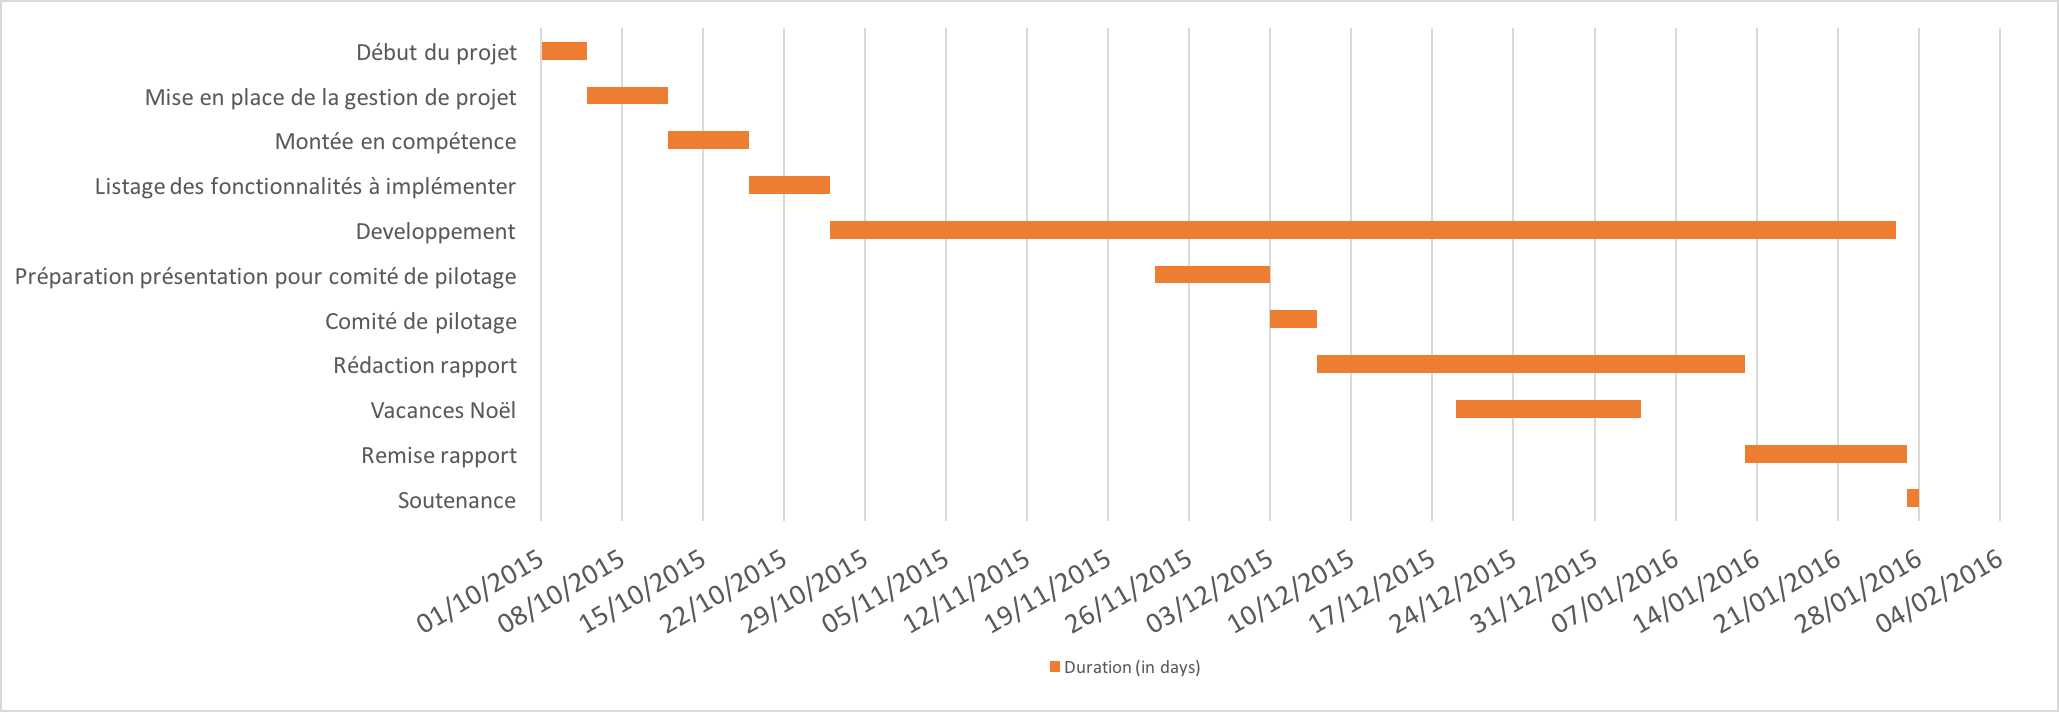
\includegraphics[scale=0.5]{img/gantt.png}
    \caption{Gantt diagram}
    \label{gantt}
\end{figure}

\subsubsection{Sprints}

\begin{center}
\begin{tabular}{|l|l|}
  \hline
  Sprint & Task\\
  \hline
  0 & Learning Big Data and Spark \\
    & Finding the use cases to develop \\ \hline
  1 & Deploying Apache Spark \\
    & Setting up real-time video processing \\
    & Exploring the Twitter API \\ \hline
  2 & Twitter mining with Spark \\
    & Real-time video processing with Spark \\ \hline
  3 & Twitter analysis \\
    & Facebook mining \& analysis \\
    & Forums mining \& analysis \\
    & Data visualization \\
  \hline
\end{tabular}
\end{center}

\subsubsection{Burndown chart}

\begin{figure}[h!]
    \centering
    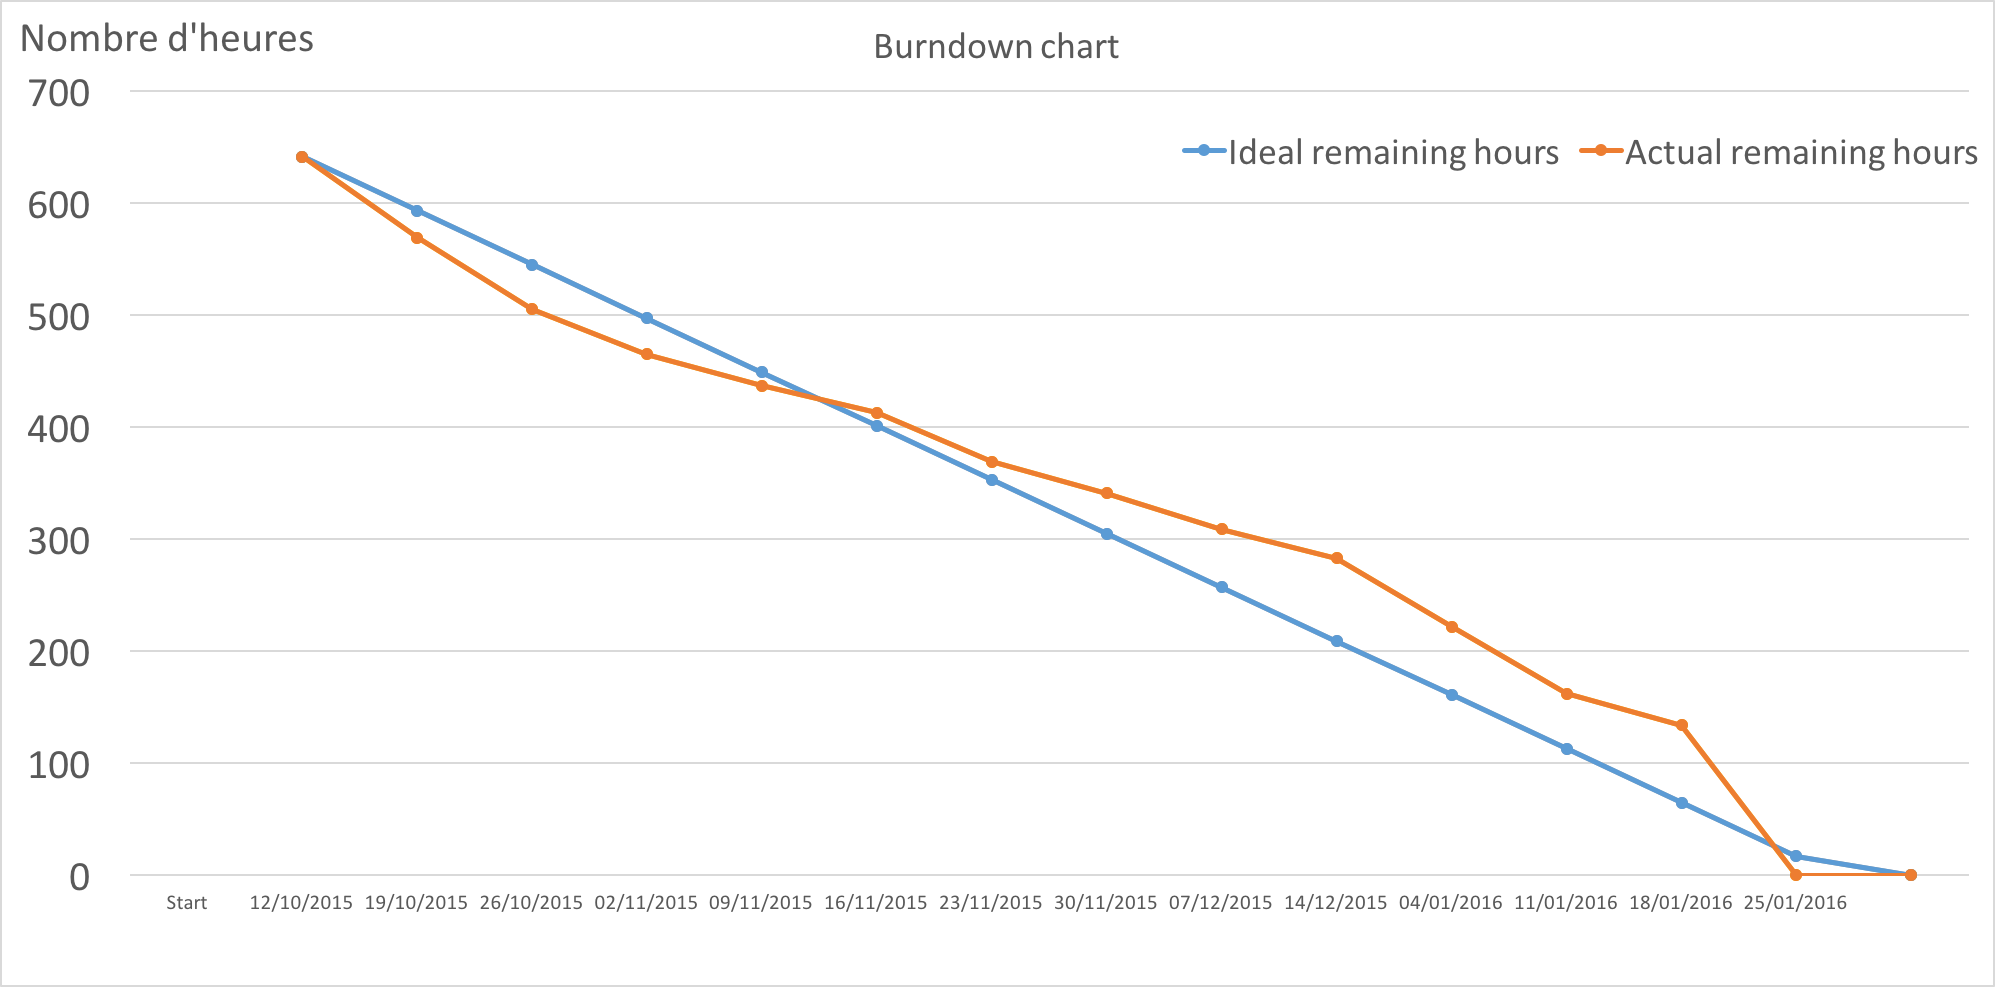
\includegraphics[scale=0.5]{img/burndown.png}
    \caption{Burndown chart}
    \label{burndown}
\end{figure}

\end{document}